\documentclass[conference]{IEEEtran}

\usepackage[utf8]{inputenc}
\usepackage[T1]{fontenc}
\usepackage{silence}\WarningsOff[latexfont]

\usepackage{listings}

\usepackage{amsmath}
\usepackage{bm}
\usepackage{dsfont}
\usepackage{amssymb}

\RequirePackage{tikz}[2010/10/13]
\usetikzlibrary{arrows,automata,calc,intersections,patterns,decorations.pathmorphing,decorations.pathreplacing}

\usepackage{graphicx}
\usepackage{cite}
\usepackage{url}
\usepackage[caption=false,font=footnotesize]{subfig}
\usepackage[binary-units,per-mode=symbol]{siunitx}
\sisetup{list-final-separator = {, and }}
\usepackage{booktabs}
\usepackage{pifont}
\usepackage{microtype}
\usepackage{textcomp}
\usepackage[american]{babel}
\usepackage[noabbrev,capitalise]{cleveref}
\usepackage{xspace}
\usepackage{hyphenat}
\usepackage{bm}
\usepackage[draft,inline,nomargin,index]{fixme}
\fxsetup{theme=color}
\usepackage{grffile}
\usepackage{xfrac}
\usepackage{multirow}
\usepackage{color} %red, green, blue, yellow, cyan, magenta, black, white
\definecolor{mygreen}{RGB}{28,172,0} % color values Red, Green, Blue
\definecolor{mylilas}{RGB}{170,55,241}
\RequirePackage{xstring}
\RequirePackage{xparse}
\RequirePackage[index=true]{acro}
\NewDocumentCommand\acrodef{mO{#1}mG{}}{\DeclareAcronym{#1}{short={#2}, long={#3}, #4}}
\NewDocumentCommand\acused{m}{\acuse{#1}}
\usepackage{upquote}

\begin{document}

\title{
    Learning a Rule\\
    \large Neural Networks and Computational Intelligence - Practical Assignment II
}

\author{
    \IEEEauthorblockN{Samuel Giacomelli}
    \IEEEauthorblockA{\small Student Number: S3546330 \\ s.giacomelli@student.rug.nl}
    \and
    \IEEEauthorblockN{Davide Pedranz}
    \IEEEauthorblockA{\small Student Number: S3543757 \\ d.pedranz@student.rug.nl}
}

\maketitle

\begin{abstract}
    Perceptrons are devices used to solve binary classification problems.
    Multiple algorithms were proposed in the literature to train a perceptron.
    In this assignment, we implement the MinOver training algorithm and measure its generalization error.
    We run simulations for datasets of different sizes and with different grades of noise.
    We compare the performances of the MinOver algorithm with the Rosenblatt one implemented in the last assignment.
\end{abstract}

\acresetall

\section{Introduction}
\label{sec:introduction}

Perceptrons are devices used to solve binary classification problems.
A perceptron tries to learn a hyperplane that divides the training examples in $2$ groups, depending on their label.
In general, if the dataset is linear separable, there is an infinite number of hyperplanes that perfectly separates the examples based on their labels.
The MinOver algorithm \cite{minover} tries to find the hyperplane with the maximum stability, i.e. maximize the distance of the closest examples from the hyperplane.

In this assignment, we implement the MinOver training algorithm and measured its generalization error on a linearly separable dataset as a function of the rate between the number of examples and their dimension.
We also compare its performances with the Rosenblatt algorithm \cite{rosenblatt} implemented in the previous assignment.
Finally, we introduce different degrees of noise in the datasets and observe the performances of both algorithms.

\cref{sec:theory} introduces the MinOver training algorithm.
\cref{sec:implementation} describes the implementation of the various experiments.
\cref{sec:evaluation} discusses the obtained results.
Finally, \cref{sec:conclusion} summarizes the most interesting results.

\section{Theory}
\label{sec:theory}

This time the focus was to find the perceptron of \textbf{maximum stability}, which means trying to maximize the margin between the
weight vector and the closest input label, or in other words trying to approximate to the teacher perceptron $\bm{\mathsf{w}}^*$.
The stability is therefore defined exactly as the distance mentioned former using the formula [\ref{eq:perceptron-stability}].

The dataset used is slightly different from the one of the Rosenblatt algorithm and the difference consists in defining the labels
as the sign of the dot product between the input and the vector that represents the teacher perceptron (i.e. the result of the
classification performed by the teacher perceptron for each input) (Formula [\ref{eq:labels_definition}]). 

The stability is calculated for every input vector contained in the dataset and, after finding all the values of $\kappa$,
the minimum is searched (Formula [\ref{eq:minimum_lookup}]) and a Hebbian update (Formula [\ref{eq:hebbian_update}]) is performed using the input vector
respect to that the perceptron has the minimum stability, the in order to maximize the value of that property.

This procedure is iterated over the number of epochs $n_{max}$ and stopped before reaching that value just if the last update
corresponds to a zero update (i.e. $\bm{\mathsf{w}}(t+1) = \bm{\mathsf{w}}(t)$). 

\begin{equation} \label{eq:labels_definition}
    S^\mu = sign(\bm{\mathsf{w}} \cdotp \xi^\mu)
\end{equation}

\begin{equation} \label{eq:perceptron-stability}
    \kappa^\mu = \frac{\bm{\mathsf{w}} \cdotp \xi^\mu S^\mu_R}{\lvert \bm{\mathsf{w}} \rvert}
\end{equation}

\begin{equation} \label{eq:minimum_lookup}
    \kappa^{\mu(t)} = \min_\nu \left \{ \kappa^{\nu(t)} =  \frac{\bm{\mathsf{w}} \cdotp \xi^\mu S^\mu_R}{\lvert \bm{\mathsf{w}} \rvert} \right \}
\end{equation}

\begin{equation} \label{eq:hebbian_update}
    \bm{\mathsf{w}}(t+1) = \bm{\mathsf{w}}(t) + \frac{1}{N} \xi^{\mu(t)} S^{\mu(t)}_R
\end{equation}
\section{Implementation}
\label{sec:implementation}

\subsection{Training and Test Set}
In different experiments we use a different number of training examples.
Given the original dataset $\mathbb{D} = \{ \varepsilon_\mu, \tau(\varepsilon_\mu)\}_{\mu=1}^M$ (with $M = 5000$), we create the training $\mathbb{D}_{train}$ and test set $\mathbb{D}_{test}$ as follows:
\begin{equation*}
    \begin{split}
        \mathbb{D}_{train} &= \{ \varepsilon_\mu, \tau(\varepsilon_\mu)\}_{\mu=1}^P, \\
        \mathbb{D}_{test} &= \{ \varepsilon_\mu, \tau(\varepsilon_\mu)\}_{\mu=Q}^M,
    \end{split}
\end{equation*}
with $Q > P$.
Since we choose $P \in [1, 2000]$ in different experiments, we fix $Q = 2001$ for all experiments, in order to always test on the same dataset. 

\subsection{Stochastic Gradient Descent}
The first step of our implementation of Stochastic Gradient Descent is to initialize the weights' vectors with random values and then normalize them to have unit norm $||w_j|| = 1$.
It is important to initialize the weights randomly in order to avoid symmetry problems:
since the weights gradient and the update rule is the same for all hidden unit, the updates at each epoch are also the same, which causes all units to learn the same final weights and reduces the representation power of the network.
Then, we perform a given number of updates:
at each iteration, we randomly select an example $\nu$ from the training dataset, compute the gradient with respect to the weights (see \cref{sub:gradients}) and update them according to \cref{eq:weights-update}.

At regular intervals (i.e. after a fixed number of iterations), we compute the error on both the entire training and the test sets, as shown in \cref{eq:cost-total}.

\section{Evaluation}
\label{sec:evaluation}
If not differently specified, all experiments discussed in this section are run with the following parameters: $N = 500$, $n_{max} = 200$, $n_D = 100$ and $c = 0$.

\subsection{Storage Capacity}
\label{subsec:capacity}
\begin{figure}[t]
	\centering
	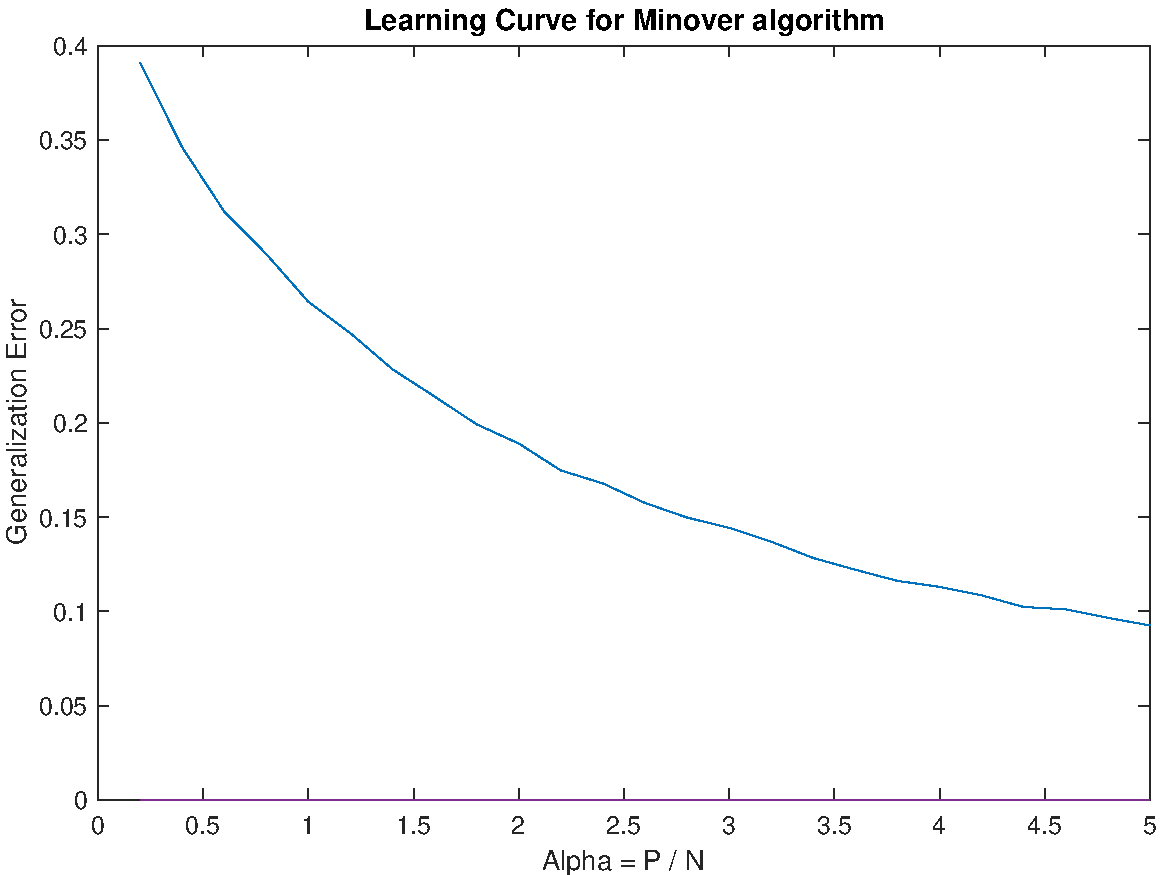
\includegraphics[width=\columnwidth]{figures/base}
    \caption{Storage success rate of a Rosenblatt perceptron as a function of $\alpha = P / N$. The experiments use $N = 500$, $n_{max} = 200$ and $n_D = 100$.}
	\label{fig:base}
\end{figure}
\cref{fig:base} shows the results of the base experiment.
The x-axis represent different values of $\alpha = P / N$, while the y-axis the success rate $Q_{l.s.}$.
As expected, the function looks like a step function from $1$ to $0$.
For $\alpha \approx 1.7$, the success rate $Q_{l.s.}$ drops from $1$ to $0$ very quickly. 

The value of $\alpha$ for which the function drops is called storage capacity of the perceptron.
For $N \to \infty$ (very large number of examples) and $n_{max} \to \infty$ (no limit on the maximum number of training iterations), the theoretical storage capacity of the Rosenblatt perceptron is $\alpha = 2$.

\subsection{Number of Iterations}
\label{subsec:epochs}
\begin{figure}[t]
	\centering
	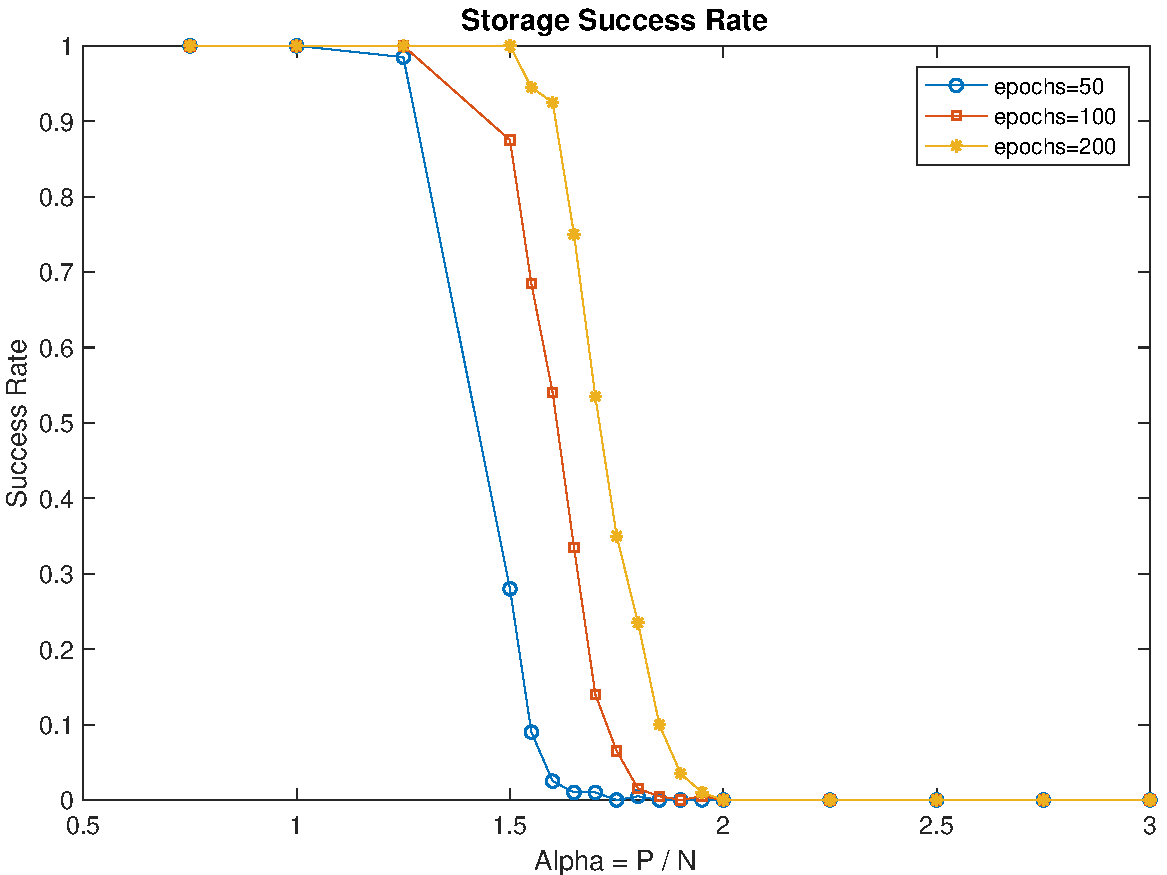
\includegraphics[width=\columnwidth]{figures/multiple_epochs}
    \caption{Storage success rate of a Rosenblatt perceptron as a function of $\alpha = P / N$ for different values of $n_{max}$.}
	\label{fig:multiple_epochs}
\end{figure}

The difference between the theoretical value and the experimental one are mainly due to the limited number of training iterations.
\cref{fig:multiple_epochs} gives an experimental proof of this statement:
for a very small number of iterations (eg. $n_{max} = 10$), the step is close to $\alpha = 1$, while for higher values of iterations the step moves closer and closer to the theoretical value $\alpha = 2$ found with \cref{eq:prob-lin-sep-alpha}.
The theoretical result still remains far from the practical one because of the limited size of input's dimension $N$.

\subsection{Number of Dimensions}
\label{subsec:dimensions}
\begin{figure}[t]
	\centering
	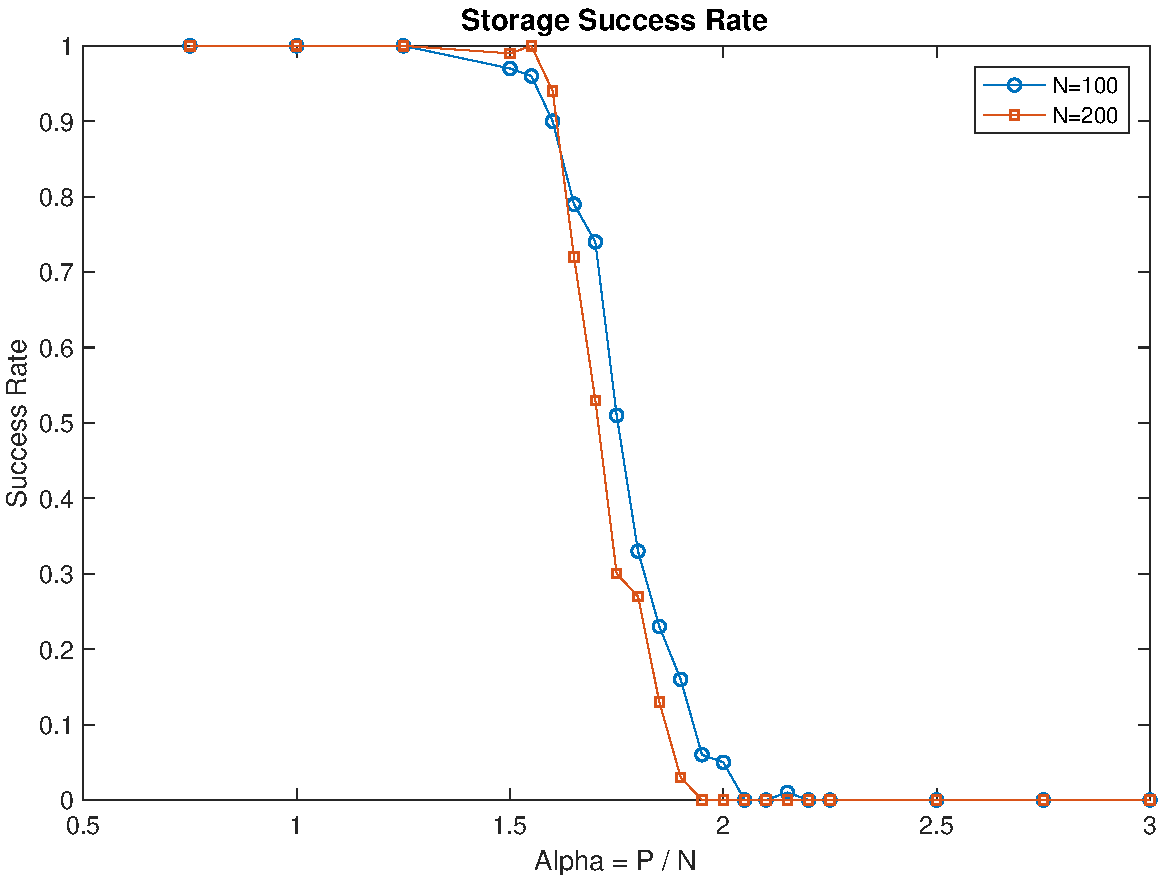
\includegraphics[width=\columnwidth]{figures/multiple_n}
    \caption{Storage success rate of a Rosenblatt perceptron as a function of $\alpha = P / N$ for different values of $N$.}
	\label{fig:multiple_n}
\end{figure}
The theoretical results are valid for $N \to \infty$.
However, real datasets have a limited number of features.
\cref{fig:multiple_n} shows the behaviour of the perceptron for different values of $N$.
For high values of $N$, the shape of the success rate $Q_{l.s.}$ as a function of $\alpha$ is similar to a step function.
For small values of $N$, the function looks like a smoothed step function:
the smaller $N$ is, the higher is the smoothing.

\subsection{Weight Update Criterion}
\label{subsec:c}
\begin{figure}[t]
	\centering
	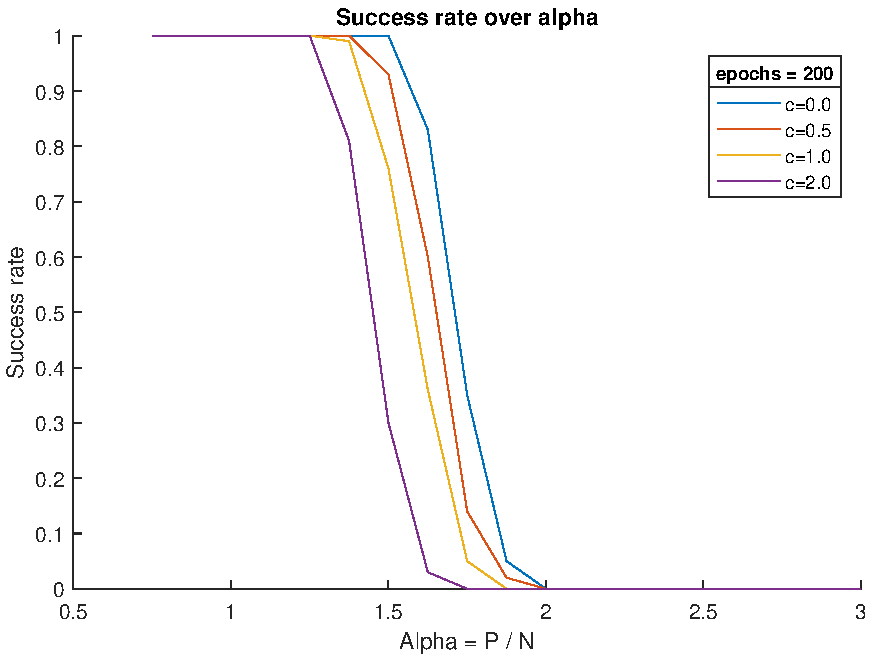
\includegraphics[width=\columnwidth]{figures/bonus_2_c}
    \caption{Storage success rate of a Rosenblatt perceptron as a function of $\alpha = P / N$ for different values of $c$.}
	\label{fig:multiple_c}
\end{figure}
\cref{fig:multiple_c} shows the effect of changing the values of $c$ in the training procedure of the perceptron.
For higher values of $c$, the curve is shifted to the left.
Since an example $\xi^\mu$ is considered correctly classified only when its local potential is greater than $c$ ($E = \mathsf{\bm{w}} \cdot \xi^\mu S^\mu > c$), the potential only depends on $\mathsf{\bm{w}}$ for a fixed $\xi^\mu$ and the update of $\mathsf{\bm{w}}$ is fixed for a given wrong classified example, the perceptron will need a higher number of updates to increase the norm of $\mathsf{\bm{w}}$ and make the local potentials higher than a threshold $c > 0$.
Formally, we can show that the value of $c > 0$ is irrelevant (provided the perceptron is trained long enough):
\begin{equation*}
	\mathsf{\bm{w}}_1 : \{E_1^\mu \geq c\}_{\mu = 1}^{P} \Leftrightarrow \mathsf{\bm{w}}_2 = \lambda \mathsf{\bm{w}}_1 : \{E_2^\mu \geq c\}_{\mu = 1}^{P}, \lambda > 0
\end{equation*}

\begin{figure}[t]
	\centering
	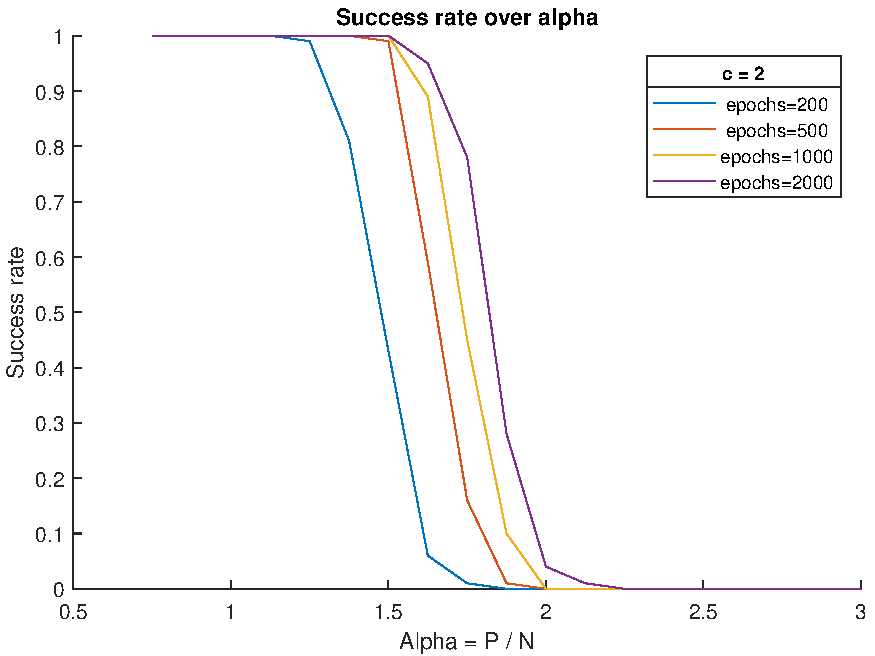
\includegraphics[width=\columnwidth]{figures/bonus_2_epoch}
    \caption{Storage success rate of a Rosenblatt perceptron as a function of $\alpha = P / N$ for different numbers of iterations with fixed value of $c=2$.}
	\label{fig:fixed_c_multiple_epoch}
\end{figure}
To give an empirical proof of this, we fix the value of $c$ and train the perceptron for different number of iterations $n_{max}$.
We expect to see the curve shifted to the left for small $n_{max}$, and approximate a step function centered in $\alpha = 2$ for big $n_{max}$.
\cref{fig:fixed_c_multiple_epoch} shows that the results of the experiment confirm our hypothesis.

\begin{figure}[t]
	\centering
	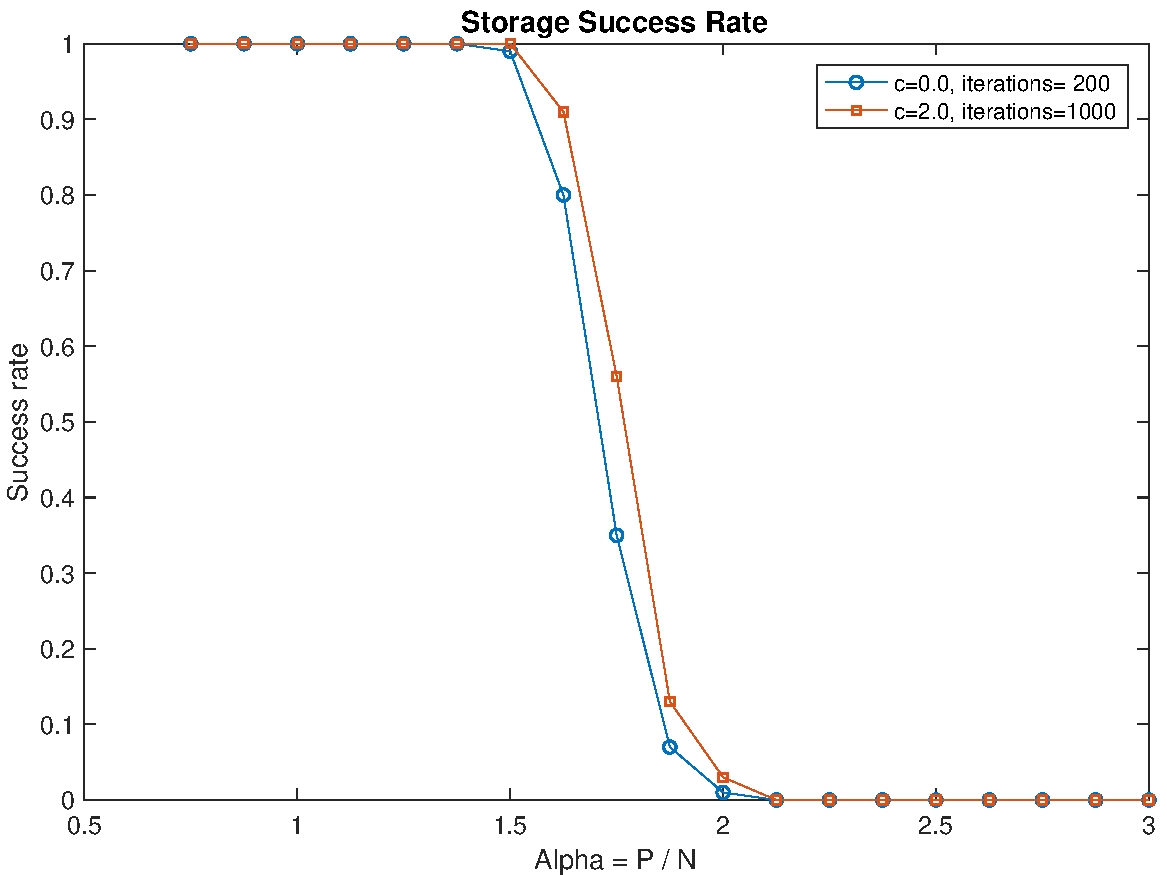
\includegraphics[width=\columnwidth]{figures/bonus_2_c_epoch}
    \caption{Storage success rate of a Rosenblatt perceptron as a function of $\alpha = P / N$ for different numbers of iterations and $c$.}
	\label{fig:multiple_c_multiple_epoch}
\end{figure}
\cref{fig:multiple_c_multiple_epoch} compares the curves for $c = 0$ and $c = 2.0$ for different values of $n_{max}$:
by increasing $n_{max}$, the curve is ``pushed'' towards the right, contrasting the effect of the increased value of $c$.
We can somehow see $c$ as a simple version of the learning rate that is used in more complex neural networks: it ``regulates'' the speed of the training.

\subsection{Inhomogeneous Hyperplanes}
\label{subsec:homogeneous}
\begin{figure}[t]
	\centering
	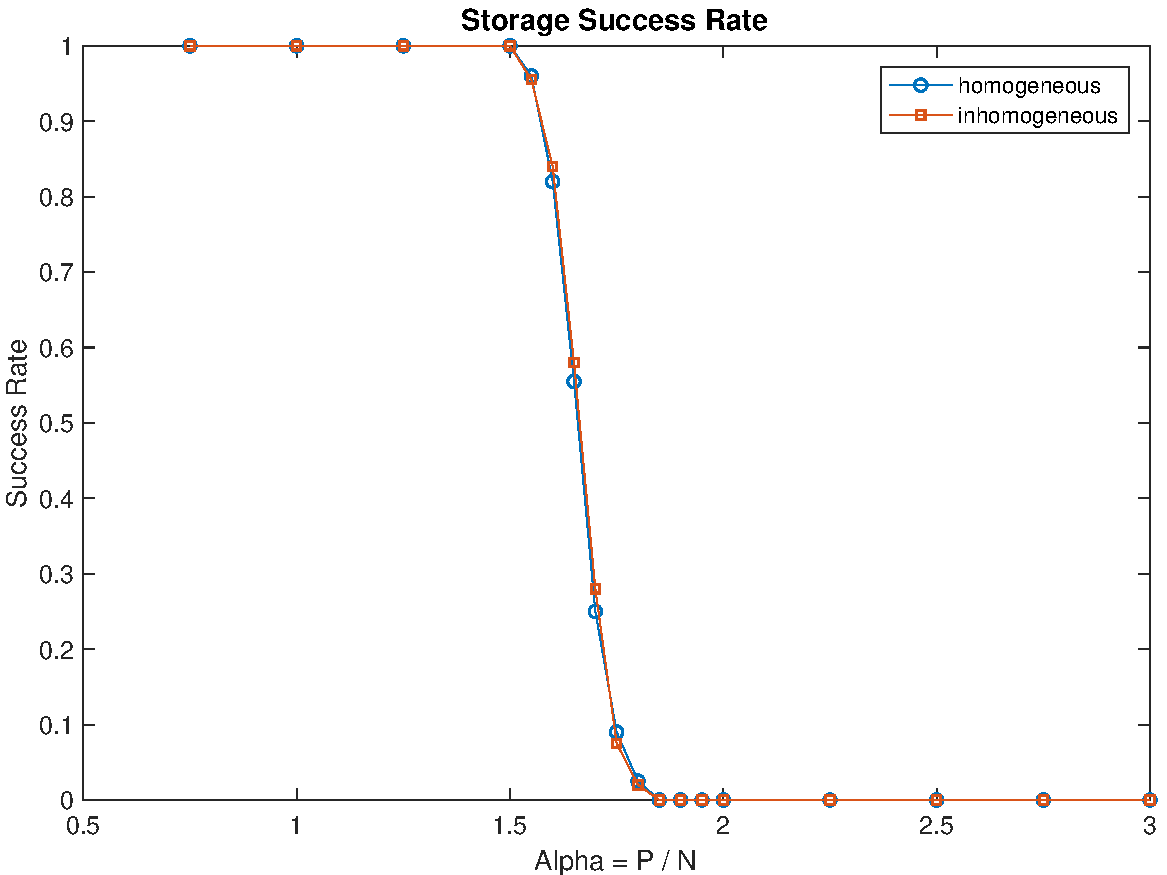
\includegraphics[width=\columnwidth]{figures/homogeneous}
    \caption{Storage success rate of a Rosenblatt perceptron and its inhomogeneous version for $N = 500$ as a function of $\alpha = P / N$.}
	\label{fig:homogeneous}
\end{figure}
We run an experiment to verify the behaviour of $Q_{l.s.}$ by allowing inhomogeneous hyperplanes:
we train both a normal and modified perceptron for $N = 500$.
\cref{fig:homogeneous} shows the results of the experiment.
As expected, the success rate $Q_{l.s.}$ of the inhomogeneous perceptron is slightly higher than homogeneous one.
However, the difference is not significant, since data points follow a normal distribution $\xi^\mu_j \sim \mathcal{N}(0,\,1)$ and are therefore distributed around the origin.

The problem of finding an inhomogeneously solution in $R^{N}$ can be solved by finding a homogeneously solution in $R^{N + 1}$.
In a second experiment, we compare the success rate $Q_{l.s.}$ of an inhomogeneous perceptron for $N = 500$ with an homogeneous perceptron for $N = 501$.
\cref{fig:homogeneous_n_n1} shows the result of this experiment.
As expected, the success rates for the $2$ perceptrons are very close to each other.

\begin{figure}[t]
	\centering
	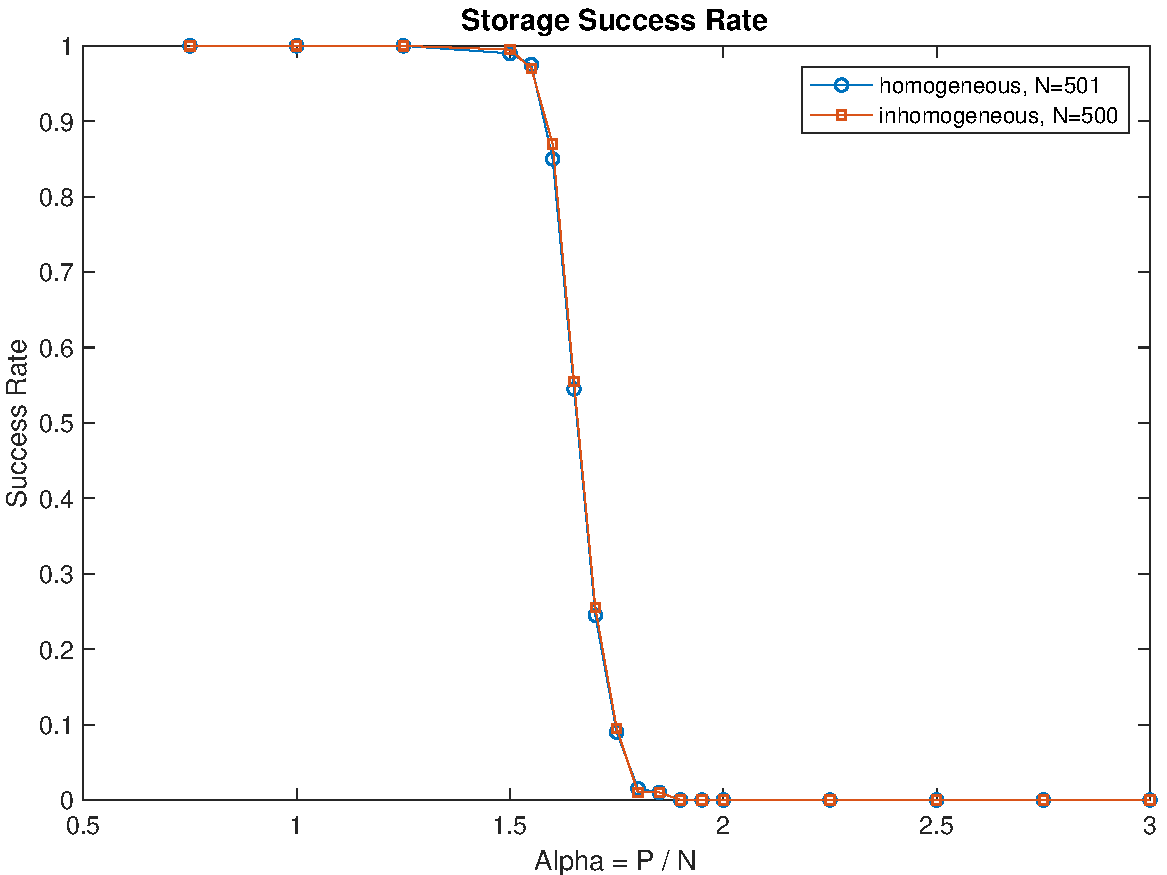
\includegraphics[width=\columnwidth]{figures/homogeneous_n_n1}
    \caption{Storage success rate of a homogeneous Rosenblatt perceptron for $N = 501$ and its inhomogeneous version for $N = 500$ as a function of $\alpha = P / N$.}
	\label{fig:homogeneous_n_n1}
\end{figure}

\section{Conclusion}
\label{sec:conclusion}

Stochastic Gradient Descent is an effective algorithm to learn the parameters of a feed-forward neural network.
The algorithm is iterative and takes as an input the number of iterations and a learning rate:
it is important to choose an appropriate value for both these parameters.
If the number of iterations is too small, the algorithms does not manage to learn the optimal parameters for the network;
if the number is too big, the model may overfit the training data and have bad performances on new data.
Similarly, if the learning rate is too small, the training may take too long or even stuck in local minima;
if it is too big, the updates may be too big and the model may never reach the optimal weights.

In general, it is difficult to choose the appropriate learning rate.
In some cases it may be effective to used a time-dependent one:
for example, one may set a big learning rate at the beginning and then reduce it to make the network converge easier.
We discussed some possible strategies and their effect on our regression problem.
However, a complete discussion of the possible learning rate policies is outside the scope of this document.

\section{Workload}
The workload of this assignment was divided as follows.

\subsection{Together}
\begin{itemize}
    \item Basic implementation of the training algorithm (pair-programming)
    \item Report
\end{itemize}

\subsection{Individually}
\subsubsection{Samuel Giacomelli}
\begin{itemize}
    \item Implementation of alternative learning rate policies
\end{itemize}
\subsubsection{Davide Pedranz}
\begin{itemize}
    \item Test of the network for different dimensions of the dataset
    % \item Accurate plots of the errors
\end{itemize}

\bibliographystyle{IEEEtran}
\bibliography{references}

\newpage
\onecolumn
\lstset{
    language=Matlab,%
    basicstyle=\fontsize{9}{11},
    breaklines=true,%
    morekeywords={matlab2tikz},
    keywordstyle=\color{blue},%
    morekeywords=[2]{1}, keywordstyle=[2]{\color{black}},
    identifierstyle=\color{black},%
    stringstyle=\color{mylilas},
    commentstyle=\color{mygreen},%
    showstringspaces=false,%without this there will be a symbol in the places where there is a space
    numbers=left,%
    numberstyle={\tiny \color{black}},% size of the numbers
    numbersep=0pt, % this defines how far the numbers are from the text
    linewidth=\columnwidth,
    emph=[1]{for,end,break},emphstyle=[1]\color{blue}, %some words to emphasize
}

\begin{appendices}
    \section{Matlab code}
    \subsection{Weights' Gradients}
    \begin{lstlisting}[language=Matlab] 
        function [g1, g2] = gd(example, tau, w1, w2)
    
            tanh_w1 =  tanh(example * w1);
            tanh_w2 = tanh(example * w2);
            sigma = tanh_w1 + tanh_w2;
            
            g_comp =  (sigma - tau) * example';
            g1 = g_comp * (1 - (tanh_w1^2));
            g2 = g_comp * (1 - (tanh_w2^2));
        end
    \end{lstlisting}
\end{appendices}


\end{document}
